\section{Ultraschallmodul HC-SR04} \label{sec:hc-sr04}
Das Ultraschallmodul HC-SR04 ist ein sehr verbreitetes Modul. Die Popularität
dieses Moduls ist gegeben durch die folgenden Eigenschaften:
\begin{itemize}
	\item unteres Preissegment (<30 CHF)
	\item Mittlerer Messbereich (2 - 400cm)
	\item Digitales Interface (TTL)
	\item Geringer Energiebedarf (75mW)
	\item Einfache Ansteuerung
\end{itemize}

\subsection{Prüfeinrichtung}
Für die Prüfung des Ultraschallmoduls ist ein projektnahes Umfeld erstellt 
worden im Elektroniklabor B332b. Hierzu ist ein freistehender Tisch 
aufgestellt worden in Richtung des Ultraschallmoduls (siehe Abbildung 
\ref{fig:testaufbau_hcsr04}). Auf diesem ist ein passender Eimer platziert
worden. Dieser hat die folgenden Eckdaten:

\begin{table}[h!]
	\centering
	\begin{tabular}{l l}
		Eigenschaft		& Wert \\
		\hline
		Durchmesser oben	& 38cm \\
		Durchmesser unten	& 33cm \\
		Höhe 			& 48cm \\
		Farbe 			& Schwarz (matt) \\
		Material		& Kunststoff \\
		Hersteller		& Helit \\
		Typ			& 61062
	\end{tabular}
	\caption{Testeimer Eckdaten}
	\label{tab:testeimer}
\end{table}

Um auch eine gewisse Relevanz und statistische Macht zu erreichen, sind 
sämtliche Prüfungen auch statistisch analysiert worden mit mindestens tausend
Einzelmessungen. Hierzu sind die Geräte des Elektroniklabor verwendet worden.
Dabei diente ein Frequenzgenerator als Ansteuerung und ein Digitales 
Speicheroszilloskop als Messmittel, welches auch gleich die statistische
Auswertung durchführte.

\begin{figure}[h!]
	\centering
	\begin{subfigure}[b]{0.45\textwidth}
		\includegraphics[width=\textwidth]{../../fig/HC-SR04_01.jpg}
		\caption{Testspielfeld}
	\end{subfigure}
	\begin{subfigure}[b]{0.45\textwidth}
		\includegraphics[width=\textwidth]{../../fig/HC-SR04_02.jpg}
		\caption{Befestigung Ultraschallmodul}
	\end{subfigure}
	\caption{Testaufbau}
	\label{fig:testaufbau_hcsr04}
\end{figure}

\subsection{Messgenauigkeit}
Um die Messgenauigkeit zu ermitteln ist der Testeimer dirket in Messrichtung
des Ultraschallmoduls aufgestellt worden zu verschiedenen Abständen. Dieser
Test zeigte auf, dass die Reichweite des Moduls ledglich 170 beträgt mit dem
gegebenen Aufbau. Dies liegt deutlich unter dem idealen Wert aus dem 
Datenblatt.

Ein Referenzversuch mit einer Sperrholzplatte zeigte auf, dass das 
Signalrauschen deutlich verringert wird im Vergleich zum Testeimer. 
Bei einem Abstand vom 180cm wurde ein mittlerer Impuls von 10.45ms mit einer
Standardabweichung von 9.7$\mu$s gemessen.

\begin{comment}
\begin{table}[h!]
	\centering
	\begin{tabular}{r r r}
		$s$ [cm] & $t_i$ (mean) [ms] & $t_j$ [us] \\
		\hline
		50 	& 2.987	& 2.4 \\
		60	& 3.503 & 2.4 \\
		70	& 4.060	& 10 \\
		80	& 4.766	& 24 \\
		90	& 5.230	& 10 \\
		100	& 5.807	& 11 \\
		110	& 6.413	& 13 \\
		120	& 7.040	& 16 \\
		130	& 7.722	& 22 \\
		140	& 8.229	& 16 \\
		150	& 8.854	& 15 \\
		160	& 9.500 & 43 \\
		170	& 10.06	& 22 \\
		180	& n.a.	& n.a. \\
	\end{tabular}
	\caption{Messgenauigkeit HC-SR04}
	\label{tab:messgenauigkeit}
\end{table}
\end{comment}

\begin{figure}[h!]
	\centering
	\begin{subfigure}[b]{0.45\textwidth}
		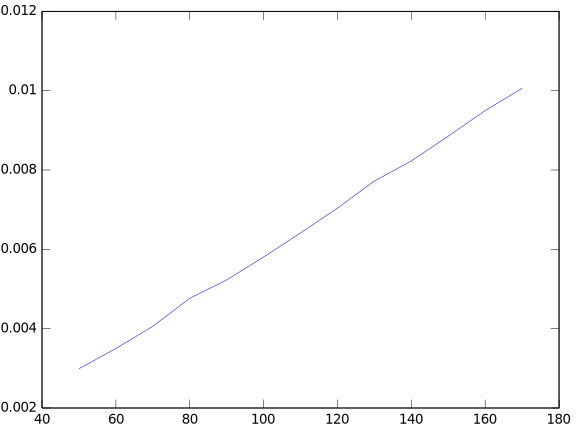
\includegraphics[width=\textwidth]{../../fig/hc-sr04_accuracy.pdf}
		\caption{Impuls Mittelwert}
		\label{fig:impuls_mean}
	\end{subfigure}
	\begin{subfigure}[b]{0.45\textwidth}
		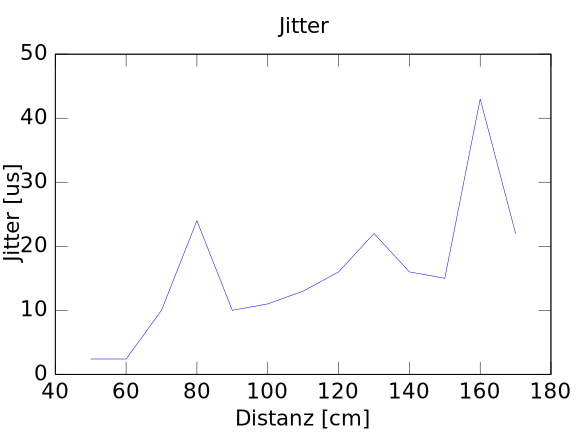
\includegraphics[width=\textwidth]{../../fig/hc-sr04_jitter.pdf}
		\caption{Jitter (Standardabweichung)}
	\end{subfigure}
	\caption{Messergebnisse der Impulsmessung}
\end{figure}

\subsection{Messempfindlichkeit}
Die Messung der Messempfindlichkeit beschreibt, wie das Modul Objekte erfassen
kann, welche nicht direkt anvisiert werden. Hierzu sind Messungen jeweils in 
5$^\circ$ Schritten durchgeführt worden. Der notierte Wert ist jener, bei
welchem das Modul den Testeimer gerade noch erkennt, d.h. bei kleineren
Distanzen wird der Testeimer erkannt.

Interessant ist hier, dass das Ultraschallmodul einen blinden Bereich aufweist
bei welchem der Testeimer nicht erkannt wird. Dieser Bereich liegt zwischen 
einem Winkel vom 25$^\circ$-30$^\circ$ und zu einer Distanz von 75-90cm.

\begin{figure}[h!]
	\centering
	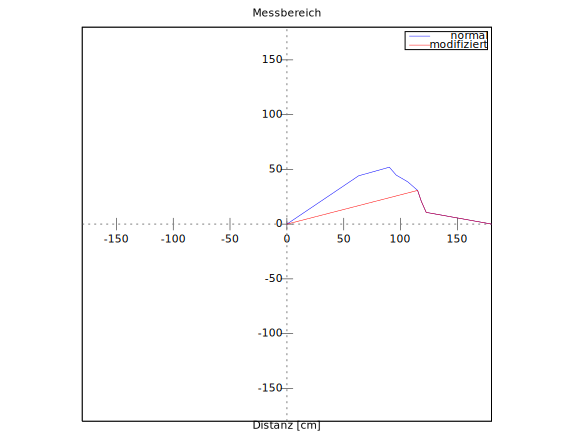
\includegraphics[width=0.8\textwidth]{../../fig/hc-sr04_range.pdf}
	\caption{Seitliche Messempfindlichkeit}
	\label{fig:sideresponse}
\end{figure}

Als einfacher Versuch zur Eingrenzung des Messbereichs ist je ein 
selbsterstelltes Papierrohr mit einer Länge von 3cm mittels eines 
Kupferdrahtes auf die Sonden des Ultraschallmoduls fixiert worden. 
Die Testreihe wurde dann in gleicher Weise wiederholt und zeigte, dass
sich der Messbereich deutlich redizuert auf ca. 15$^\circ$. Dieser Effekt 
kann extrapoliert werden in der Weise, dass längere Röhren zu einem weiteren 
Einschnüren des Messbereich führen sollten. Diese Hypothese wurde jedoch
keinem Test unterzogen.

\begin{figure}[h!]
	\centering
	\includegraphics[width=0.8\textwidth]{../../fig/HC-SR04_08.jpg}
	\caption{Modifiziertes Ultraschallmodul}
\end{figure}

\subsection{Fazit}
Das Ultraschallmodul HC-SR04 bietet auch unter projektnahen Bedingungen 
eine hohe Linearität (siehe Abbildung \ref{fig:impuls_mean}).
Dies bedeutet, dass sich das Modul sehr wohl eignet für eine direkte 
Distanzmessung mit geringer Toleranz. Dies funktioniert jedoch nur in einem
Bereich von bis zu 170cm, was deutlich unter dem Datenblattwert liegt und knapp
ist für die geplante Applikation.

Die weiteren Messungen zeigten zudem, dass das Modul insbesondere bei 
inderekter Messung des Testeimers deutliche Schwierigkeiten aufweist. Die 
polare Darstellung dieser Messergebnisse zeigt, dass ein eigentlicher 
Messkegel nicht vorhanden ist (siehe Abbilgung \ref{fig:sideresponse}).
Dies eliminiert den Einsatz des Moduls für das Abtasten des Spielfelds nach
dem Zielobjekt, insbesondere dann, wenn zu dem nichtidealen seitlichen
Messverhalten des Moduls auch Reflexionen und dadurch ausgelöste 
Interferenzen berücksichtigt werden. Für das Abtasten des Spielfeldes 
gilt es ein Messverfahren zu verwenden, welches entweder unempfindlich ist
gegenüber Reflexionen und sonstigen Interferenzen von Aussen oder sehr
punktuell operieren kann, was Reflexionen von vornherein ausschliesst.
Ein typischer Vertreter solcher Messmittel sind Laserbasierte Geräte.
